%! Author = user
%! Date = 25/01/2021

% Preamble
\documentclass[11pt]{article}

\begin{document}

    \section{Design Principle}
    Design principles are guidelines to assist in your object-oriented design.

    \subsection{Encapsulate what varies}
    Identify the aspects of your application that vary and separate them from what stays the same.
    \begin{itemize}
        \item Look for code that changes with every new requirements. We can see which behavior needs to be pulled out
        and separated from the stuff that does not change.
        \item Alter or extend the code that varies without affecting code that doesn't vary.
        \item Basis of almost every design pattern. All patterns tend to provide a way to let some part of your system
        vary independently on the other parts.
        \item Pay attention to how each pattern makes use of this principle.
    \end{itemize}

    \subsection{Favor composition over inheritance}
    Identify the aspects of your application that vary and separate them from what stays the same. Also know as has-a
    is better than is-a.
    \begin{itemize}
        \item Inheritance is a powerfull technique that avoid code duplication. However it is a technique that can
        bet easily overused. It is also a technique that can lead to designs that are far too rigged and not extensible.
        \item Is-a is a relationship of inheritance e.g. dog is a animal.
        \item Has-a is a relationship of composition e.g. dog has a owner. Compisition can be a powerfull alternative
        to inheritance. How can we switch from Is-a to Has-a:
        \begin{itemize}
            \item Instead of a CoffeeWithButter is-a Coffee.
            \item what about a Coffee Has-a condiment?
        \end{itemize}
        \item We can add any number of condiments easily at runtime.
        \item Implementing new condiments by adding a new class.
        \item No code duplication.
        \item Avoid class explosion.
        \item Instead of inheriting behavior, we can compose our objects with new behaviors.
        \item Composition often gives us more flexibility, even allows behavior changes at runtime.
        \item Composition is a common techniques used in design patterns.
    \end{itemize}

    \subsection{Loose Coupling}
    Components should be independent, relying on knowledge of other component as little as possible.
    \begin{itemize}
        \item When two classes interact, changes in one class should not force changes on the other one.
        \item Loose coupling reduces the dependency between components. Keeping designs loosely coupled helps us to build
        object-oriented systems that can handle change well.
        \item Simple technique to achieve loose coupling: abstracting away a concrete type into an interface. This
        is a technique your are going to see reoccur over and over again in good design.
        \item A good example of loose couple is the Observer pattern.
    \end{itemize}

    \subsection{Program to Interfaces, Not Implementations}
    Where possible, components should use abstract classes or interfaces instead of a specific implementation.
    \begin{itemize}
        \item "program to an Interface" really means "program to a super/abstract type".
        \item The point is to be able to exploit polymorphism by programming to a super type so that your
        actual runtime object isn't locked into you code.
        \item The "new" operator only work on concrete types. Doesn't that violates this principle? Here we can
        make use of creational design patterns.
        \item Encourages us to use interfaces/abstract classes when possible, rather than concrete classes.
        \item This principle frees classes from knowledge of concrete types.
        \item Improve extensibility and maintainability.
    \end{itemize}

    \subsection{Single Responsiblity Principle}
    Classes should have only one reason to change.
    \begin{itemize}
        \item Look at the change in your class: Are parts of it changing while other parts are not?
        \item Change only matters if it really happens. So apply Single Responisiblity only when the need is real, or you
        are just creating complexity.
    \end{itemize}

    \subsection{Open/Close Principle}
    Object-Oriented designs should be open for extension, but closed for modification.
    \begin{itemize}
        \item An example of this is using composition to allow behavior extension of a class, while protecting the existing
        (proven) code of the class from modification.
        \item A design pattern that make use of this principle is the strategy pattern. In the duck example we are able
        to add new duck behaviors without changing the duck class.
        \item Improve maintainability and extensibility of a design.
    \end{itemize}

    \subsection{Liskov's Substitution Principle}
    You should always be able to substitute subtypes for their base class.
    \begin{itemize}
        \item Using Inheritance the wrong way, can lead to undesired behavior when substituting the baseclass with the
        subsclass.\\
        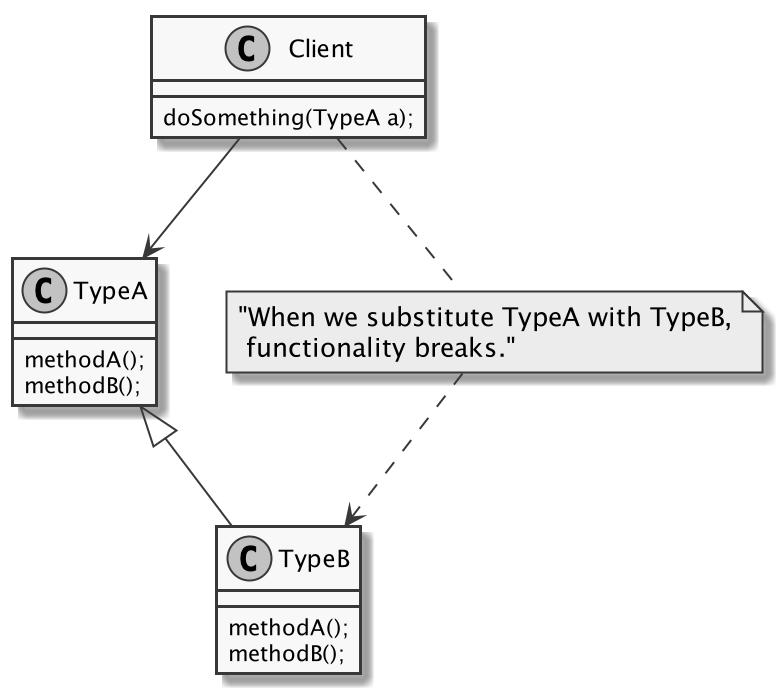
\includegraphics[scale=0.2]{liskov_substitution_principle}
        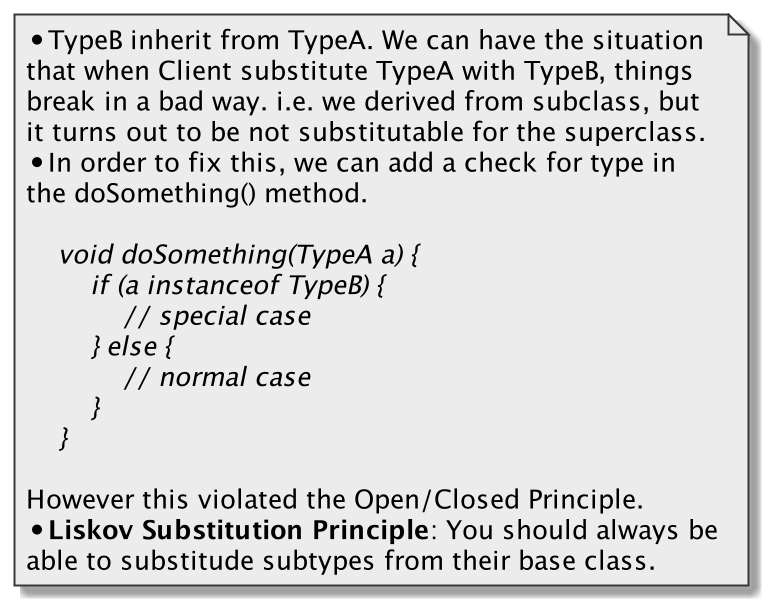
\includegraphics[scale=0.2]{liskov_substitution_principle2}
        \item Example is the Rectangle and Square class. When Square is derived from Rectangle, it violated the Liskov
        Substitution Principle, since changing the length of a Square also changes the width of the Square. This side-effect
        is not in the rectangle super class. i.e. a Square class can not substitude the Rectangle class.
        \item Don't assume that the IsA principle will always result in hierarchies that adhere to this principle. You
        will need to consider how substitutable a base class is for it's supertype as well.
        \item To adhere to this principle, we can use techniques like design by contract.
    \end{itemize}

    \subsection{Interface Segregation Principle}
    Classes should not be forces to depend on methods that they don't use.
    \begin{itemize}
        \item Cohesion: How strong are the relationship between an interface's methods. i.e. We say a class is highly
        cohesive if their methods are related.
        \item Think able the client that uses the interface. Is the client going to use all the method in the interface? if yes
        then the interface has high cohesion.
        \item Highly cohesive interfaces leads to software that is easier to maintain and easier to extend.
        \item Segregate Interfaces needed to keep them focussed and cohesive. i.e. you free the clients from methods they
        are not intrested in. \\
        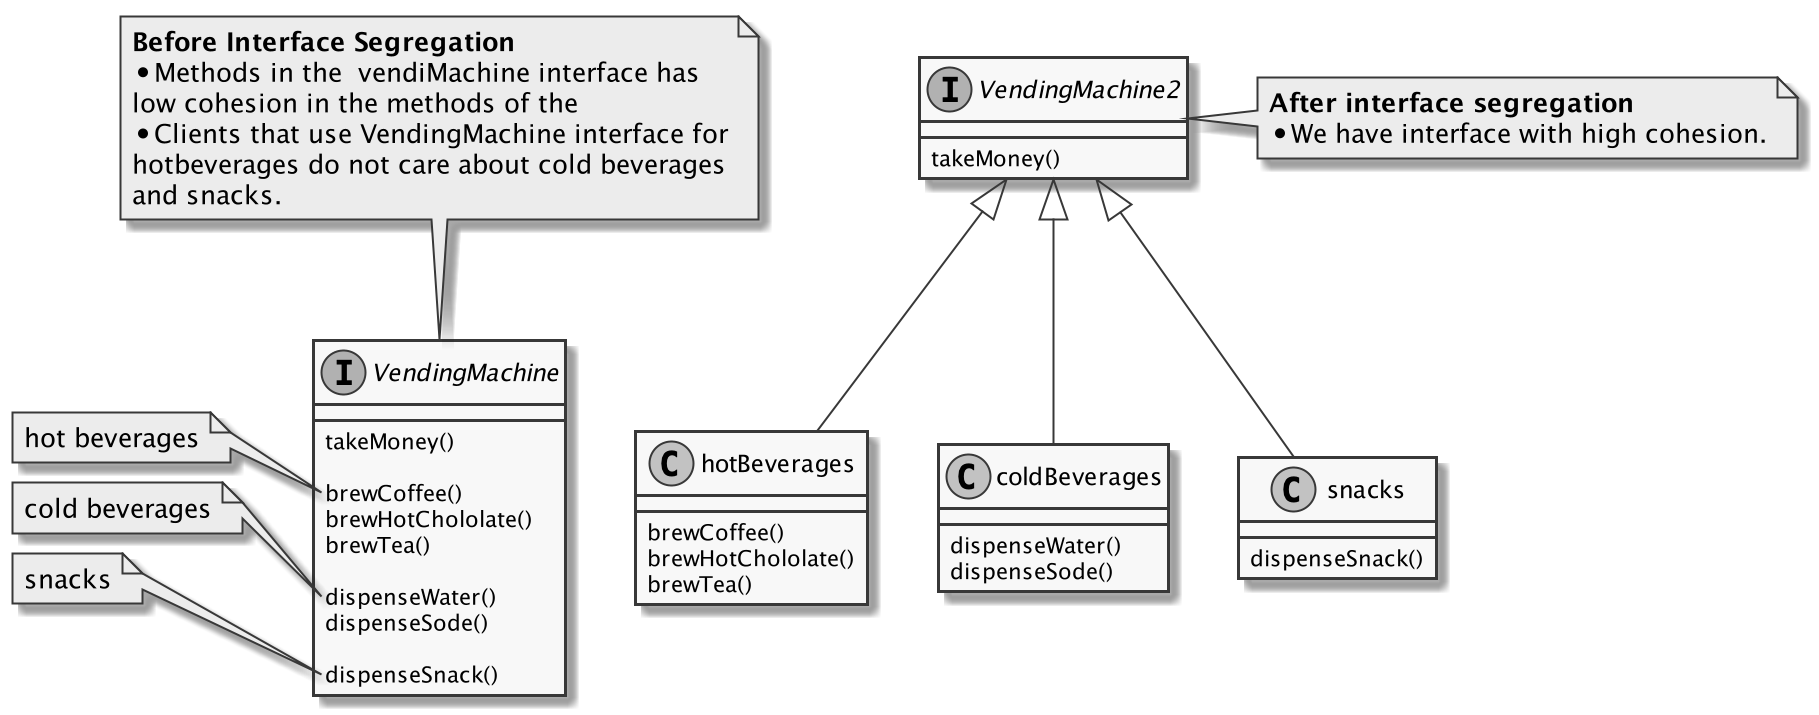
\includegraphics[scale=0.2]{interface_segregation_principle}
    \end{itemize}

    \subsection{Dependency Inversion Principle}
    High-level modules should not depend on low-level modules
    \begin{itemize}
        \item Typical Object-Oriented Thinking: We take a problem, and we factor it into a high-level set of components
        (the policy-makers) that depend on low-level components, who are carrying out the real work. The problem with
        this approach is that is tightly couples our high-level components to our low-level ones.
        \item A symptom of tight coupling is that it's difficult to reuse the high-level components with a different implementation
        of the low-level component.
        \item Dependency Inversion Principle:
        \begin{enumerate}
            \item High-level components should not depend on low-level components. Both should depend on abstractions.
            \item Abstractions should not depend on details. Details should depend on abstractions.
        \end{enumerate}
        \item What is high-level policy? It is the abstraction that underlies the application. i.e. In our example, it
        is a remote control that can control anything. \\
        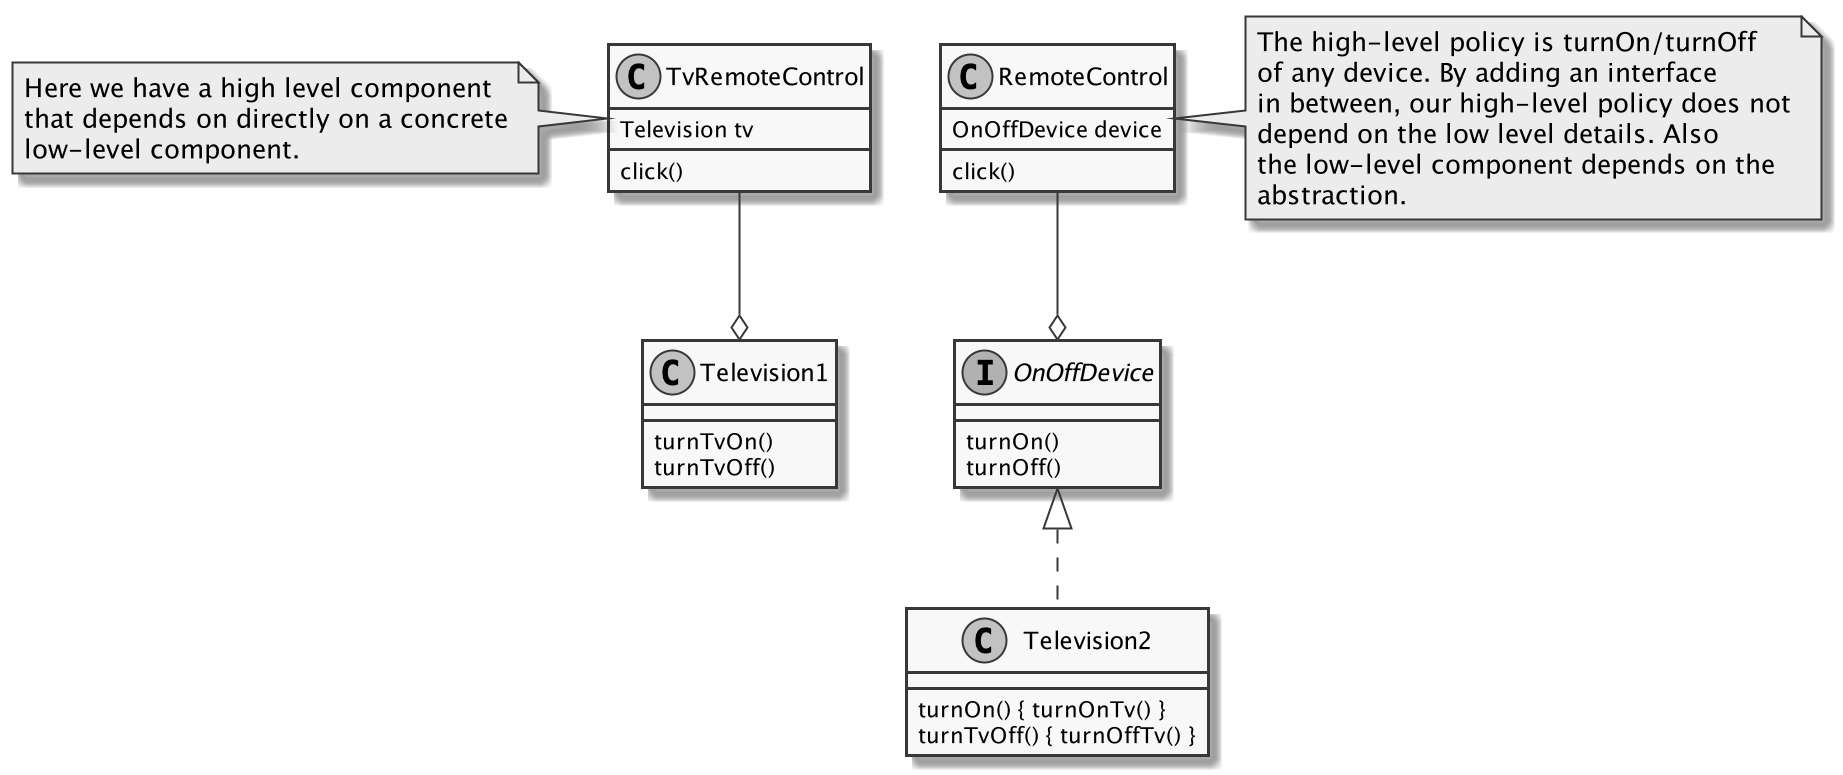
\includegraphics[scale=0.2]{dependency_inversion_principle}
        \item This principle frees our high-level components from being dependent on the details of the low-level
        components.
        \item It helps design software that is reusable and resilient against changes.
        \item Abstraction allow details to remain isolated from each other.
    \end{itemize}

\end{document}
